\chapter{ADC tracking}
In this experience we built an 8-bit ADC tracking with the output switching from 0 and 5 volt (TTL logic).

\section{Materials}
\begin{itemize}
\item Resistors, capacitors
\item Power supply RIGOL DP831A
\item 5V power supply NI myDAQ
\item Waveform generator RIGOL DG1032
\item Multimeter RIGOL DM3068
\item Digital counter (from previous experiment)
\item DAC08
\item 8-bit LED viewer
\item Comparator LM311
\end{itemize}
The resistors used were all with an uncertainty of 5\%

\section{Experimental setup}
First of all we tested our DAC08 powering it with \(\pm\)15V and setting the input current in the $+V_{Ref}$ pin to 2mA: this was achieved by tuning the voltage coming from the RIGOL power supply and a resistor of 2.2k\(\Omega\). In order to clear as much as possible the bias current effects, we used another identical resistor between the $-V_{Ref}$ pin and ground, we also added a 10nF capacitor between the COMP pin and -15V to optimize the behaviour of the component.\\
Since we used TTL logic and only one output, we put to ground both the $V_{LC}$ and the $\overline{I_{Out}}$ pins.\\
At this point we had an output current, but we desired an output voltage: for that reason we added a 2081.7\(\pm\)0.4\(\Omega\) resistor between the $I_{Out}$ pin and ground. We then tested the component with various different inputs and measured its resolution. 
\\Once done these measurements we connected the counter circuit from last experiment as the DAC08 input and we verified the ``sawtooth'' output of the DAC. Finally we connected this output to a comparator together with the input voltage to be converted, obtained from the -15V power supply voltage with a 5.6k\(\Omega\) resistor and a 5k\(\Omega\) trimmer (therefore freely variable), and used this new output as the $\overline{Up}$/Down counter input. We tested the circuit with the D flip flop between the counter and the $\overline{Up}$/Down input and without it. Capacitors 0.1\(\mu\)F were added to all the connections with power supply.\\
We chose different analog voltage at different clock frequencies and visualized them with the 8-bit LED viewer. In this way we verified the correct working of the circuit.

\begin{figure}[H]
\centering
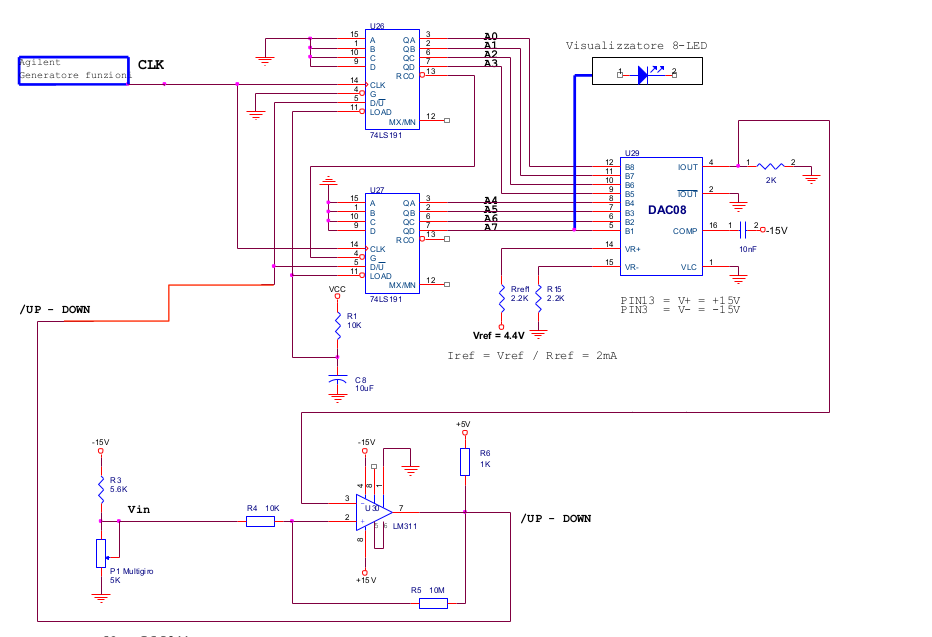
\includegraphics[width=.8\textwidth]{12/circuit.png}
\caption{Circuit used}
\end{figure}

\section{Data Analysis}
Once mounted the DAC08, we tested its output with different configurations of the input. The results are shown in table 11.1 \\

\begin{table}[H]
\centering
 \begin{tabular}{lllllllllll}
 \toprule
  Range Fraction & B1 & B2 & B3 & B4 & B5 & B6 & B7 & B8 & $I_{out}$ (measured) & $V_{out}$ (measured) \\
 \midrule
  FULL RANGE & 1 & 1 & 1 & 1 & 1 & 1 & 1 & 1 & 1.9870\(\pm\)0.0011 mA & -4.1358\(\pm\)0.0003 V \\
  HALF-SCALE +LSB & 1 & 0 & 0 & 0 & 0 & 0 & 0 & 1 & 1.0057\(\pm\)0.0006 mA & -2.09378\(\pm\)0.00018 V \\
  HALF-SCALE & 1 & 0 & 0 & 0 & 0 & 0 & 0 & 0 & 0.9979\(\pm\)0.0006 mA & -2.07775\(\pm\)0.00018 V \\
  HALF-SCALE  -LSB & 0 & 1 & 1 & 1 & 1 & 1 & 1 & 1 & 0.9892\(\pm\)0.0006 mA & -2.05968\(\pm\)0.00018 V \\
  ZERO-SCALE +LSB & 0 & 0 & 0 & 0 & 0 & 0 & 0 & 1 & 8.08\(\pm\)0.03 \(\mu\)A & -16.807\(\pm\)0.006 mV \\
  ZERO-SCALE & 0 & 0 & 0 & 0 & 0 & 0 & 0 & 0 & 0.33\(\pm\)0.03 \(\mu\)A & -0.744\(\pm\)0.005 mV \\
 \bottomrule
 \end{tabular}
\caption{Test DAC08: measurements}
\end{table}  

\begin{table}[H]
\centering
 \begin{tabular}{lllllllllll}
 \toprule
  Range Fraction & B1 & B2 & B3 & B4 & B5 & B6 & B7 & B8 & $I_{out}$ (theoretical) & $V_{out}$ (theoretical)\\
 \midrule
  FULL RANGE & 1 & 1 & 1 & 1 & 1 & 1 & 1 & 1 & 1.992\(\pm\)0.004 mA & -4.147\(\pm\)0.008 V \\
  HALF-SCALE +LSB & 1 & 0 & 0 & 0 & 0 & 0 & 0 & 1 & 1.008\(\pm\)0.002 mA & -2.098\(\pm\)0.004 V \\
  HALF-SCALE & 1 & 0 & 0 & 0 & 0 & 0 & 0 & 0 & 1.000\(\pm\)0.002 mA & -2.082\(\pm\)0.004 V \\
  HALF-SCALE  -LSB & 0 & 1 & 1 & 1 & 1 & 1 & 1 & 1 & 0.992\(\pm\)0.002 mA & -2.065\(\pm\)0.004 V \\
  ZERO-SCALE +LSB & 0 & 0 & 0 & 0 & 0 & 0 & 0 & 1 & 7.8125\(\pm\)0.016 \(\mu\)A & -16.26\(\pm\)0.03 mV \\
  ZERO-SCALE & 0 & 0 & 0 & 0 & 0 & 0 & 0 & 0 & 0\(\pm\)0 \(\mu\)A & 0\(\pm\)0 mV \\
 \bottomrule
 \end{tabular}
\caption{Test DAC08: expected values given $I_{Ref}=2.000$\(\pm\)0.004mA, $R_{out}=2081.7$\(\pm\)0.4\(\Omega\)}
\end{table}  

Comparing the results in these last 2 tables, we can see that the measurements are sufficiently compatible with the expected values (with the only exeption of the zero-scale that theoretically should be zero with no uncertainty at all).\\
We can as well measure the resolution of our converter: it is the least difference that we can distinguish between two different outputs. Making an average, we come to the result of 1LSB = 16.72\(\pm\)0.12 mV, that is distant from its theoretical value of 16.26\(\pm\)0.03 mV of only 3\(\sigma\). \\
After we connected the DAC08 to the counter, we verified the signal tracking and we "captured" feature of our system, we were able to observe the response to a 0.3V continue input, using a 30Hz clock frequency and setting the oscilloscope time scale to 20ms/div. We got a ladder in the first part, beginning from 0V and approaching to the input voltage with subsequent steps at the clock frequency, each step modifiyng the output of a value equal to the resolution of the circuit. As the output overtook the signal in input, it began decreasing and increasing one step after another, keeping the medium value equal to the input one.
We can see the graphic obtained in figure 11.2\\


\begin{figure}[H]
\centering
\begin{minipage}{.48\textwidth}
\centering
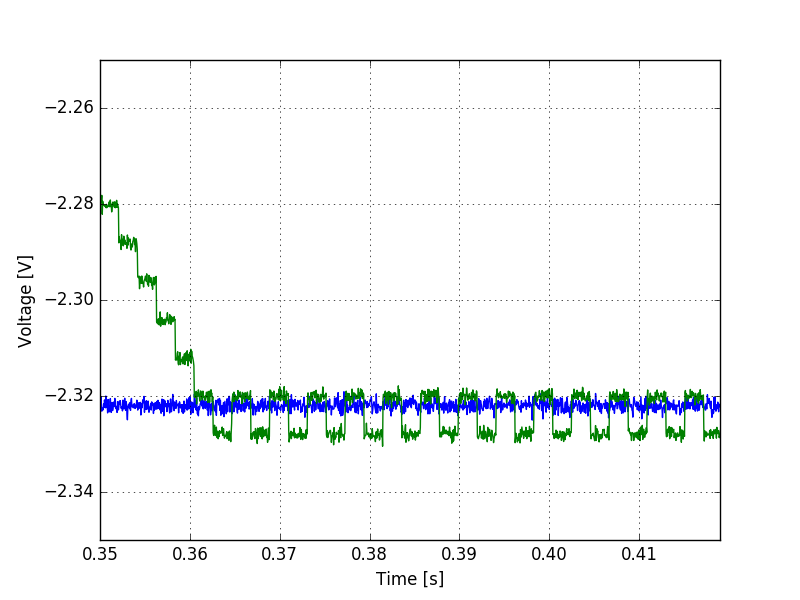
\includegraphics[width=\textwidth]{12/good.png}
\caption{signal tracking without flip flop}
\end{minipage}\,
\begin{minipage}{.48\textwidth}
\centering
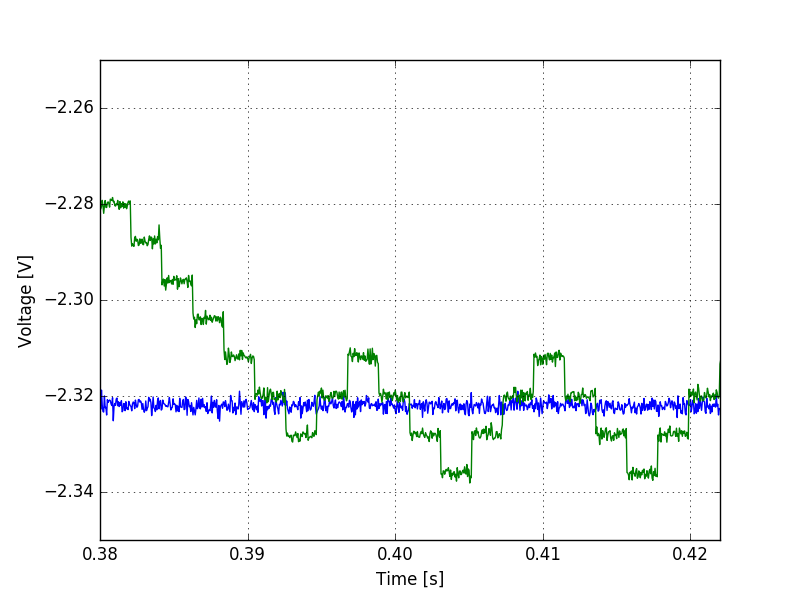
\includegraphics[width=\textwidth]{12/good2.png}
\caption{signal tracking with flip flop}
\end{minipage}
\end{figure}

As we can see in the second figure, where we used the flip-flop in the previous experiment, the output was fluctuating more than one bit. This happened because the message for counting up or down arrived to the counter one clock pulse after it left the comparator and not at the same time.
